\documentclass[11pt,a4paper]{article}
\usepackage[T1]{fontenc}
\usepackage[utf8]{inputenc}
\usepackage{lmodern}
\usepackage[margin=2.3cm]{geometry}
\usepackage{amsmath}
\usepackage{graphicx}
\usepackage{booktabs}
\usepackage{siunitx}
\usepackage{xcolor}
\usepackage[colorlinks=true,linkcolor=black,citecolor=blue!50!black,urlcolor=blue!50!black]{hyperref}
\usepackage{url}
\graphicspath{{figures/}}
\newcommand{\Eads}{E_\mathrm{ads}}

\begin{document}

% ------------------------------------------------------------------ title page
\begin{titlepage}
\centering
{\large Bogoliubov Laboratory of Theoretical Physics\\ Joint Institute for Nuclear Research\par}
\vspace{2.5cm}
{\Large FINAL REPORT ON THE\\ INTEREST PROGRAMME\par}
\vspace{1.5cm}
{\LARGE\bfseries Adsorption of mercury on Au(111):\\ machine-learning interatomic potentials\\ versus density functional theory\par}
\vspace{2.5cm}
\begin{flushright}
\textbf{Supervisor:}\\ Dr Miroslav Ilia\v{s}\\
\textbf{Co-supervisor:}\\ Dr Dipayan Sen\\[1em]
\textbf{Student:}\\ Ne\c{s}et Ko\c{c}kar, T\"urkiye\\ Department of Physics, Ankara University\\[1em]
\textbf{Participation period:}\\ 26 October -- 4 December 2026, Wave 15
\end{flushright}
\vfill
{\large Dubna, 2026\par}
\end{titlepage}

\tableofcontents
\newpage

% ------------------------------------------------------------------ abstract
\begin{abstract}
The adsorption of a single Hg atom on Au(111), the benchmark for gas-phase chemistry of copernicium on gold detectors, was computed with two universal machine-learning interatomic potentials (CHGNet, MACE-MP-0) and with plane-wave DFT (PBE and PBE-D3(BJ)) under one consistent protocol. The upstream ASE results were reproduced exactly. Both MLIPs bind Hg two to three times more strongly than the PBE level they were trained on ($\Eads(\mathrm{fcc}) = -0.94$ and $-0.77$~eV vs.\ $-0.33$~eV). This study shows that a large part of this overbinding comes from the untrained energy of the free Hg atom: its error, obtained through the Hg cohesive energy, is $+0.45$~eV for CHGNet and $+0.22$~eV for MACE. A ``far-away'' reference with Hg 10~\AA\ above the slab does not detect this error, because the atom has no neighbours inside the 6~\AA\ model cutoff. All methods agree on the site preference (fcc $\approx$ hcp $>$ bridge $>$ ontop), but the MLIPs exaggerate the site corrugation about threefold. PBE-D3 gives $\Eads = -0.69$~eV (66~kJ/mol), compared with the thermochromatographic $-\Delta H_\mathrm{ads} = 98\pm3$~kJ/mol; PBE alone gives only 32~kJ/mol.
\end{abstract}

% ------------------------------------------------------------------ 1
\section{Introduction}
Gold-covered detector surfaces are used at the Flerov Laboratory of Nuclear Reactions (FLNR) and at GSI to identify superheavy elements (SHE) chemically, one atom at a time. A volatile atom transported in a gas stream along a temperature gradient deposits where its residence time on the surface becomes long. The deposition pattern is converted by Monte-Carlo simulation into a standard adsorption enthalpy $\Delta H_\mathrm{ads}^\mathrm{Au}$~\cite{soverna2005,eichler2007,eichler2008,lens2018}. Copernicium (Cn, $Z=112$) was characterised in this way as a volatile group-12 metal with $-\Delta H_\mathrm{ads}^\mathrm{Au}(\mathrm{Cn}) = 52^{+3}_{-2}$~kJ/mol~\cite{eichler2007,eichler2013}. Its lighter homologue mercury binds more strongly, $-\Delta H_\mathrm{ads}^\mathrm{Au}(\mathrm{Hg}) = 98\pm3$~kJ/mol ($\approx 1.02$~eV)~\cite{soverna2005,lens2018}. Hg is therefore the natural benchmark system for computational methods that are later to be applied to Cn and other SHE~\cite{gaston2007,pershina2009}.

The INTEREST project~411 explores whether cheap interatomic potentials, from Lennard-Jones (LJ) to universal machine-learning interatomic potentials (MLIPs), can predict such adsorption energies. The supervisor's ASE scripts~\cite{upstream,ase} give, for a single Hg atom on Au(111), $\Eads(\mathrm{fcc}) = -0.899$~eV with CHGNet~\cite{chgnet}. CHGNet itself warns that the isolated Hg atom used as the energy reference ``will likely go wrong''. This report
(i) reproduces the upstream numbers,
(ii) re-computes them with one consistent protocol for CHGNet and MACE-MP-0~\cite{mace,macemp0},
(iii) quantifies the error caused by the isolated-atom reference, and
(iv) provides plane-wave DFT reference values (PBE and PBE-D3) with Quantum ESPRESSO~\cite{qe2009,qe2017}, compared with experiment.

% ------------------------------------------------------------------ 2
\section{Methods}
\subsection{Structural model and protocol}
All methods use the same protocol, and all settings are logged with the results:
\begin{enumerate}
\item The fcc Au lattice constant $a_0$ is optimised \emph{with each method} (Birch--Murnaghan fit). Using the ASE default $a=4.08$~\AA\ for all methods would put every method except experiment under strain.
\item Au(111) slab, $3\times3$ surface cell, 4 layers (36 Au atoms), 12~\AA\ vacuum on each side; the bottom two layers are fixed at bulk positions.
\item One Hg atom (coverage 1/9 ML) at the ontop, bridge, fcc and hcp sites. Hg relaxes only along $z$, so each site stays at its high-symmetry position. Free (unconstrained) relaxations are run separately to test site stability.
\item Relaxations stop at $f_\mathrm{max}=0.02$~eV/\AA\ (BFGS; ASE for the MLIPs, the QE-internal BFGS for DFT).
\end{enumerate}
The adsorption energy is $\Eads = E(\text{slab+Hg}) - E_\mathrm{ref}$, with four reference schemes:
\begin{itemize}
\item[\textbf{A}] $E_\mathrm{ref} = E(\text{slab}) + E(\text{Hg atom in a }15$~\AA\ box$)$, the upstream approach;
\item[\textbf{B}] $E_\mathrm{ref} = E(\text{slab + Hg fixed 10~\AA\ above the surface, same cell})$, the ``far-away'' reference;
\item[\textbf{C}] $E_\mathrm{ref} = E(\text{slab}) + E_\mathrm{bulk}(\alpha\text{-Hg}) + E_\mathrm{coh}^\mathrm{exp}(\mathrm{Hg})$, using only condensed-phase energies and the experimental cohesive energy 0.67~eV/atom~\cite{kittel};
\item[\textbf{D}] as C, but with the PBE cohesive energy computed here. For an MLIP trained on PBE data, D replaces the model's untrained free-atom energy with the PBE value, transferred through bulk Hg.
\end{itemize}
In addition, the energy of Hg above the rigid relaxed slab was scanned from 1.8 to 12~\AA\ (fcc site).

\subsection{Interatomic potentials}
\textbf{CHGNet} 0.3.0 weights~\cite{chgnet} (package 0.4.2, float32) and \textbf{MACE-MP-0 medium}~\cite{macemp0} (mace-torch 0.3.16, float64, no D3 add-on) were run through ASE~3.29 on an NVIDIA RTX PRO 4000 GPU. Both are trained on PBE(+U) Materials Project data and use a 6~\AA\ cutoff. The upstream \textbf{LJ} script uses ASE's element-blind default parameters ($\varepsilon=1$~eV, $\sigma=1$~\AA). It was run only to reproduce the upstream number and as a numerical control (Sect.~\ref{sec:upstream}).

\subsection{DFT}
Quantum ESPRESSO 7.6 (CPU, MPI, 10 ranks)~\cite{qe2009,qe2017}, PBE~\cite{pbe} and PBE-D3 with Becke--Johnson damping and the three-body term (QE \texttt{dftd3\_version=4})~\cite{d3,d3bj}. Pseudopotentials are from SSSP~1.3 precision~\cite{sssp}: Au SG15 ONCV (norm-conserving, 19 valence electrons)~\cite{oncv,sg15}; Hg GBRV ultrasoft (12 valence electrons)~\cite{gbrv}; both scalar-relativistic. Other settings: Marzari--Vanderbilt smearing 0.01~Ry~\cite{mv}, spin-unpolarised (Hg is closed-shell $6s^2$), $k$-mesh $4\times4\times1$ for the slab, $\Gamma$ only for the atom, $16^3$ for bulk Au, $12^3$ for $\alpha$-Hg, SCF threshold $10^{-8}$~Ry, force threshold $7.8\times10^{-4}$~Ry/bohr (0.02~eV/\AA). Convergence tests on a $2\times2\times3$ model (Table~\ref{tab:conv}) give:
\begin{itemize}
\item cutoffs of 50/300~Ry change $\Eads$ by $<0.3$~meV relative to 65/390 and 80/480~Ry, so 50/300~Ry was used;
\item the $k$-mesh error is about 10--15~meV;
\item vacuum (8 vs 12~\AA) changes $\Eads$ by $\le1.5$~meV and a dipole correction (computed dipole $\approx0.5$~D per Hg) by $\le4$~meV; no dipole correction was used in production.
\end{itemize}
Technical details:
\begin{itemize}
\item The fixed bottom-layer atoms carry a separate species label (same pseudopotential). This prevents QE from keeping symmetry operations, such as the inversion of the clean 4-layer slab, that map fixed onto free atoms.
\item QE's \texttt{upscale} was set to 1, so the SCF threshold stays at $10^{-8}$~Ry during relaxations.
\item Calculations ran on the CPU build (10 MPI ranks) or the GPU build of QE~7.6 (1 RTX PRO 4000) with identical inputs.
\item The QE force criterion acts on each Cartesian component, the ASE criterion on the norm of the force vector.
\end{itemize}

\begin{table}[h]
\centering
\caption{DFT convergence tests (PBE unless noted) on a rigid $2\times2\times3$ test model at 1/4~ML; energies in eV. The $k$-meshes $4\times4$, $6\times6$, $9\times9$ on the $2\times2$ cell correspond to about $2.7\times2.7$, $4\times4$ and $6\times6$ on the $3\times3$ production cell.}
\label{tab:conv}
\small
\begin{tabular}{llrrr}
\toprule
Test & Setting & $E_\mathrm{ads}$(fcc) & $E_\mathrm{ads}$(ontop) & $\Delta E_\mathrm{fcc-ontop}$\\
\midrule
cutoff & 50/300 Ry & -0.2717 & -0.1126 & -0.1591\\
cutoff & 65/390 Ry & -0.2718 & -0.1126 & -0.1591\\
cutoff & 80/480 Ry & -0.2716 & -0.1125 & -0.1591\\
ecutrho & 65/520 Ry & -0.2715 & -0.1123 & -0.1592\\
kmesh & $k$ 4x4x1 & -0.2578 & -0.0874 & -0.1705\\
kmesh & $k$ 9x9x1 & -0.2837 & -0.1145 & -0.1692\\
vacuum & vacuum 12 \AA & -0.2704 & -0.1111 & -0.1594\\
dipole & dipole corr. & -0.2685 & -0.1089 & -0.1597\\
D3 & PBE-D3(BJ) & -0.6535 & -0.4696 & -0.1839\\
\bottomrule
\end{tabular}

\end{table}

% ------------------------------------------------------------------ 3
\section{Results}
\subsection{Reproduction of the upstream scripts}\label{sec:upstream}
The supervisor's scripts~\cite{upstream} were run unmodified (copies verified by checksum). The results are identical to the logged values to all printed digits: CHGNet fcc $-0.8986$ / ontop $-0.7069$~eV on both CPU and GPU, MACE ontop/bridge/fcc/hcp $-0.5678/-0.7084/-0.7288/-0.7249$~eV, and LJ $-0.0108$~eV. The upstream CHGNet and MACE scripts differ in slab size ($3\times3\times4$ vs.\ $4\times4\times4$), number of fixed layers (2 vs.\ 1) and force threshold (0.05 vs.\ 0.005~eV/\AA), so their numbers are not directly comparable. Both use the ASE default $a=4.08$~\AA. With each model's own $a_0$ ($\approx4.17$~\AA, PBE-like) the binding is 20--50~meV stronger, and changing $f_\mathrm{max}$ between 0.05 and 0.02~eV/\AA\ changes $\Eads$ by $\le7$~meV (\texttt{results/mlip\_sensitivity.csv}). The LJ script uses element-blind ASE defaults ($\sigma=1$~\AA, $\varepsilon=1$~eV). With a self-consistent lattice constant, Hg sinks into the surface and the bridge relaxation diverges. LJ is therefore used only as a numerical control (its free-atom energy is exactly zero, so schemes A and B coincide by construction).

\subsection{Bulk properties and the isolated-atom problem}
\begin{table}[h]
\centering
\caption{Bulk reference properties. $E_\mathrm{coh}(\mathrm{Hg}) = E(\text{Hg atom}) - E(\alpha\text{-Hg})$ per atom. Experimental Au lattice constant 4.078~\AA; Hg cohesive energy from Ref.~\cite{kittel}.}
\label{tab:bulk}
\begin{tabular}{lrrrr}
\toprule
Method & $a_0$(Au) (\AA) & $B_0$(Au) (GPa) & $E_\mathrm{coh}$(Hg) (eV) & $V$($\alpha$-Hg) (\AA$^3$/atom)\\
\midrule
CHGNet & 4.171 & 129 & 0.622 & 30.3\\
MACE-MP-0 & 4.176 & 134 & 0.388 & 29.7\\
PBE & 4.150 & 142 & 0.169 & 29.7\\
PBE-D3(BJ) & 4.108 & 162 & 0.527 & 25.6\\
\midrule
Experiment & 4.078 & -- & 0.67 & --\\
\bottomrule
\end{tabular}

\end{table}

Table~\ref{tab:bulk} shows that both MLIPs reproduce the PBE description of the condensed phases: Au $a_0$ within 0.03~\AA\ and the (strongly overestimated) PBE volume of $\alpha$-Hg within 2\,\%. Their Hg cohesive energies, however, are 0.62 (CHGNet) and 0.39~eV (MACE), compared with 0.17~eV in PBE. Because the condensed phase is reproduced, the difference has to come from the free atom: relative to PBE, the energy of an isolated Hg atom is too high by $+0.45$~eV in CHGNet and by $+0.22$~eV in MACE. No isolated atoms were in the training data, so this energy is an extrapolation. CHGNet's value happens to be close to experiment (0.67~eV), but only by accident: the model should reproduce PBE, not experiment. D3 raises the PBE cohesive energy to 0.53~eV and reduces the $\alpha$-Hg volume from 29.7 to 25.6~\AA$^3$.

Scheme B does not remove this error. Figure~\ref{fig:scan} shows that both MLIP binding curves reach their asymptote at about 5.5--6~\AA, the model cutoff. A Hg atom 10~\AA\ above the surface (with periodic images 8.65~\AA\ apart) has no neighbours, and its energy is identical to that of the isolated atom: $|\Eads^\mathrm{B}-\Eads^\mathrm{A}|<0.1$~meV for all sites (Fig.~\ref{fig:schemes}, left). In DFT the same difference is $0.2$~meV for PBE and 10~meV for PBE-D3 (the dispersion tail at 10~\AA). Scheme D replaces the MLIP free-atom energy with the PBE one, transferred through bulk $\alpha$-Hg. It shifts all MLIP adsorption energies by the constant amounts shown in Fig.~\ref{fig:schemes} (right).

\begin{figure}[h]
\centering
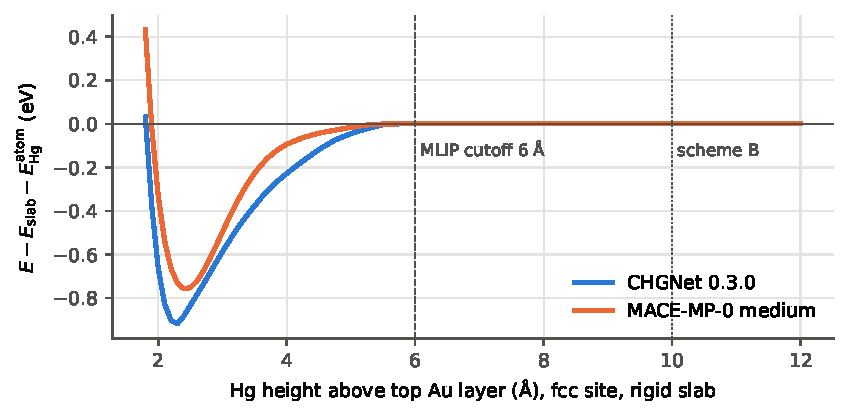
\includegraphics[width=0.85\textwidth]{fig_dissociation_scan.pdf}
\caption{Energy of Hg above the fcc site of the rigid, relaxed slab relative to slab + isolated atom (MLIPs). The curves become flat at the 6~\AA\ cutoff, so the far-away reference (dotted line) is equivalent to the isolated atom.}
\label{fig:scan}
\end{figure}

\begin{figure}[h]
\centering
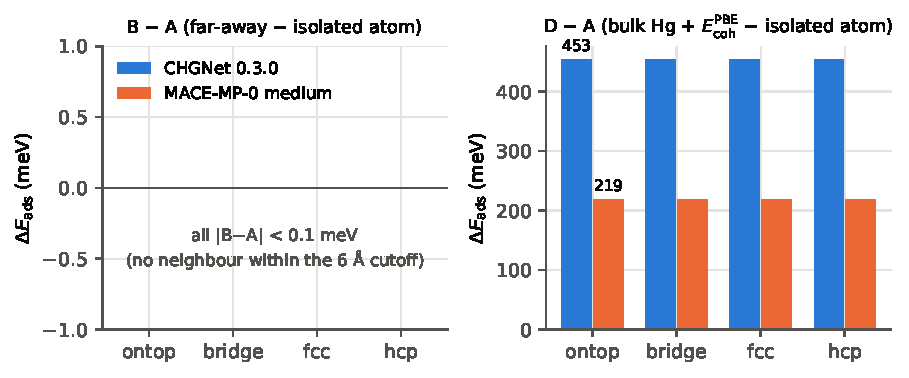
\includegraphics[width=0.9\textwidth]{fig_scheme_difference.pdf}
\caption{Change of the MLIP adsorption energies when the reference is changed. Left: far-away (B) minus isolated atom (A). Right: bulk-Hg + PBE cohesive energy (D) minus A, i.e.\ the isolated-atom error of each model.}
\label{fig:schemes}
\end{figure}

\subsection{Adsorption energies and geometries}
\begin{table}[h]
\centering
\caption{Adsorption energies of Hg on Au(111) ($3\times3\times4$, 1/9~ML) for the four reference schemes, Hg height $h$ above the mean top Au layer and shortest Au--Hg distance (from the scheme-A geometry; schemes differ only in the reference energy). D is defined for the MLIPs only. All relaxations converged.}
\label{tab:main}
\small
\begin{tabular}{llrrrrrr}
\toprule
Method & Site & \multicolumn{4}{c}{$E_\mathrm{ads}$ (eV), scheme} & $h$ (\AA) & $d_\mathrm{Au-Hg}$ (\AA)\\
\cmidrule(lr){3-6}
 & & A & B & C & D & & \\
\midrule
CHGNet & ontop & -0.734 & -0.734 & -0.782 & -0.281 & 2.53 & 2.65\\
 & bridge & -0.907 & -0.907 & -0.954 & -0.453 & 2.21 & 2.76\\
 & fcc & -0.943 & -0.943 & -0.991 & -0.490 & 2.18 & 2.83\\
 & hcp & -0.939 & -0.939 & -0.986 & -0.485 & 2.19 & 2.83\\
\midrule
MACE-MP-0 & ontop & -0.574 & -0.574 & -0.856 & -0.355 & 2.65 & 2.74\\
 & bridge & -0.748 & -0.748 & -1.030 & -0.530 & 2.43 & 2.88\\
 & fcc & -0.774 & -0.774 & -1.056 & -0.555 & 2.39 & 2.95\\
 & hcp & -0.768 & -0.768 & -1.050 & -0.549 & 2.40 & 2.96\\
\midrule
PBE & ontop & -0.266 & -0.266 & -0.767 & -- & 2.87 & 2.86\\
 & bridge & -0.315 & -0.315 & -0.816 & -- & 2.55 & 2.95\\
 & fcc & -0.333 & -0.333 & -0.834 & -- & 2.47 & 3.01\\
 & hcp & -0.333 & -0.333 & -0.834 & -- & 2.46 & 3.01\\
\midrule
PBE-D3(BJ) & ontop & -0.579 & -0.569 & -0.722 & -- & 2.79 & 2.81\\
 & bridge & -0.660 & -0.650 & -0.803 & -- & 2.49 & 2.91\\
 & fcc & -0.686 & -0.675 & -0.828 & -- & 2.43 & 2.97\\
 & hcp & -0.685 & -0.675 & -0.828 & -- & 2.42 & 2.97\\
\bottomrule
\end{tabular}

\end{table}

\begin{figure}[h]
\centering
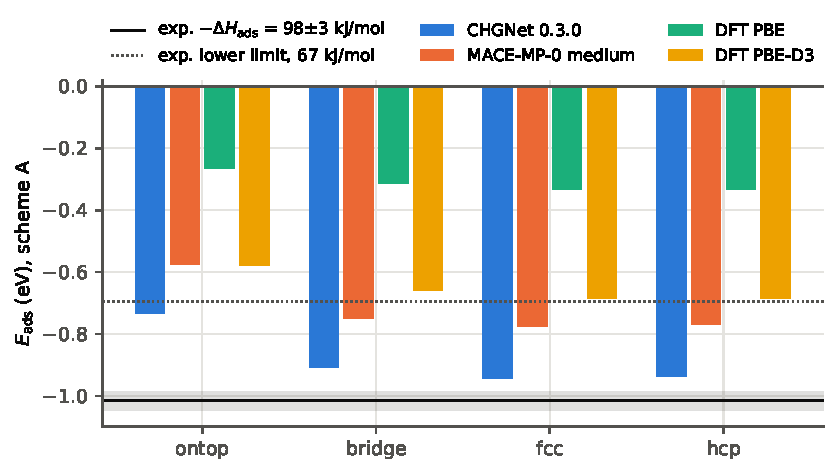
\includegraphics[width=0.9\textwidth]{fig_eads_sites.pdf}
\caption{$\Eads$ (scheme A) per site and method. Band: thermochromatographic $-\Delta H_\mathrm{ads}^\mathrm{Au}(\mathrm{Hg}) = 98\pm3$~kJ/mol~\cite{soverna2005,lens2018}; dotted: lower limit 67~kJ/mol from Ref.~\cite{lens2018}.}
\label{fig:eads}
\end{figure}

Table~\ref{tab:main} and Fig.~\ref{fig:eads} summarise the adsorption results. PBE binds Hg weakly: $-0.27$ (ontop), $-0.32$ (bridge) and $-0.33$~eV (fcc, hcp; the two hollow sites differ by 0.1~meV). PBE-D3(BJ) adds about $-0.31$ to $-0.35$~eV of dispersion, giving $-0.58$ (ontop), $-0.66$ (bridge) and $-0.69$~eV (fcc, hcp). D3 also shortens the Hg--surface distance by 0.03--0.08~\AA. Relative to PBE, the raw (scheme A) MLIP energies deviate by 0.57 (CHGNet) and 0.40~eV (MACE) on average over the four sites. After the isolated-atom correction (scheme D) the deviations drop to 0.12 and 0.19~eV. Geometrically, MACE is closer to PBE than CHGNet (mean deviation of $h$: 0.12 vs.\ 0.31~\AA; of $d_\mathrm{Au-Hg}$: 0.07 vs.\ 0.19~\AA): CHGNet places Hg 0.3~\AA\ too close to the hollow sites.

All methods predict the same order of sites, fcc $\approx$ hcp $>$ bridge $>$ ontop. However, the MLIPs exaggerate the corrugation. The ontop site lies 0.21 (CHGNet) and 0.20~eV (MACE) above fcc, compared with 0.07~eV in PBE and 0.11~eV in PBE-D3. The fcc--hcp difference is below 6~meV in all methods, i.e.\ below the accuracy of any of them. In unconstrained relaxations (\texttt{results/mlip\_site\_stability.csv}), the bridge site is a saddle point for CHGNet (Hg slides into the fcc hollow and gains 37~meV), whereas MACE keeps Hg at the bridge position.

% ------------------------------------------------------------------ 4
\section{Discussion}
\paragraph{(1) Size of the isolated-atom error.} For both MLIPs, the CHGNet warning about isolated atoms points to a real problem. Measured against PBE through the Hg cohesive energy, the free-atom energy is wrong by $+0.45$~eV (CHGNet) and $+0.22$~eV (MACE). This is 48\,\% and 28\,\% of the scheme-A adsorption energy at the fcc site. The error affects every site equally and therefore does not change the site preference, only the absolute value. A ``far-away'' reference within the same cell cannot correct it for a local model with a finite cutoff. Possible corrections are a condensed-phase reference (scheme D), or computing the free-atom energy with the DFT method the model was trained on.

\paragraph{(2) Which MLIP is closest to DFT?} For the raw (upstream-style) adsorption energy, MACE-MP-0 is closer to PBE (mean deviation 0.40 vs.\ 0.57~eV), mainly because its isolated-atom error is smaller. After the isolated-atom correction, CHGNet is closer in energy (0.12 vs.\ 0.19~eV) and reproduces the PBE ontop value to 15~meV. MACE gives clearly better geometries. Neither MLIP reaches the accuracy needed (about 0.1~eV $\approx$ 10~kJ/mol) to discriminate between adsorption enthalpies measured in thermochromatography. Even after the correction, both overbind the hollow sites by 0.16--0.22~eV relative to PBE.

\paragraph{(3) Site preference.} All four methods agree that Hg prefers the threefold hollow sites, with fcc and hcp degenerate within the accuracy of every method, followed by bridge and ontop. The MLIPs exaggerate the energy differences between sites about threefold relative to PBE and twofold relative to PBE-D3, and CHGNet turns the bridge site into a saddle point.

\paragraph{(4) DFT and experiment.} The thermochromatographic value $-\Delta H_\mathrm{ads}^\mathrm{Au}(\mathrm{Hg}) = 98\pm3$~kJ/mol~\cite{soverna2005,lens2018} corresponds to 1.02~eV. PBE (0.33~eV, 32~kJ/mol) misses two thirds of it, consistent with its poor description of Hg cohesion (0.17 vs.\ 0.67~eV). PBE-D3(BJ) gives 0.69~eV (66~kJ/mol), essentially at the lower limit of 67~kJ/mol derived from on-line chromatography in Ref.~\cite{lens2018}, but still 32~kJ/mol below the thermochromatographic value. The remaining gap is plausibly related to the factors listed in Sect.~\ref{sec:limits}: polycrystalline gold with steps and defects in experiment versus an ideal (111) terrace here, enthalpy versus 0~K energy, and the approximate treatment of relativity and dispersion. The raw CHGNet value ($-0.94$~eV) lies closest to experiment, but because of the isolated-atom error, not because of better physics.

The comparison is relevant for Cn. A method applied to Cn should first reproduce the Hg benchmark. Among the methods tested here, only dispersion-corrected DFT comes within about 30\,\% of the experimental Hg value; the out-of-the-box MLIPs cannot be used for absolute adsorption energies without correcting their free-atom reference.

% ------------------------------------------------------------------ 5
\section{Limitations}\label{sec:limits}
\begin{itemize}
\item \textbf{No spin--orbit coupling.} All DFT calculations are scalar-relativistic. SOC is small for closed-shell Hg ($6s^2$) but matters for the $6d/7p$ shells of Cn. A transfer of the protocol to Cn requires a fully relativistic treatment.
\item \textbf{Model surface.} A $3\times3\times4$ slab (1/9 ML coverage, four layers) and an ideal (111) facet. Thermochromatography probes polycrystalline gold at zero coverage, where steps and defects can bind more strongly.
\item \textbf{Energy vs.\ enthalpy.} $\Eads$ is a 0~K electronic energy. Zero-point and thermal corrections, and the mobile-adsorption model used to derive $\Delta H_\mathrm{ads}$ from experiment, are not included.
\item \textbf{Functional.} PBE lacks dispersion; D3(BJ) is an empirical correction whose Hg parameters were not fitted to metal surfaces.
\item \textbf{Numerical.} $k$-point error of about 10--15~meV (Table~\ref{tab:conv}); the MLIPs are used as released (no fine-tuning).
\end{itemize}

% ------------------------------------------------------------------ 6
\section{Conclusions}
\begin{itemize}
\item The upstream ASE/MLIP scripts were reproduced exactly, and a consistent benchmark protocol (method-specific lattice constant, identical slab, constraints and thresholds, four sites, four reference schemes) was set up for MLIPs and DFT. All scripts and raw data are provided.
\item The CHGNet isolated-atom warning is justified. The free-atom energy of Hg is too high by 0.45~eV (CHGNet) and 0.22~eV (MACE-MP-0) relative to PBE, which makes the upstream adsorption energies too negative by the same amount. A far-away reference in the same cell does not detect this for models with a 6~\AA\ cutoff; a condensed-phase (bulk Hg) reference does.
\item All methods agree on the site preference fcc $\approx$ hcp $>$ bridge $>$ ontop. The MLIPs overestimate the site corrugation about threefold, and CHGNet places Hg about 0.3~\AA\ too close to the surface.
\item PBE strongly underbinds Hg ($-0.33$~eV, 32~kJ/mol). PBE-D3(BJ) gives $-0.69$~eV (66~kJ/mol), compared with the experimental $98\pm3$~kJ/mol.
\item Next steps: fully relativistic (SOC) calculations for Cn, stepped Au surfaces, and MLIP fine-tuning on Hg/Au DFT data including the free atom.
\end{itemize}

\section*{Acknowledgements}
I thank Dr Miroslav Ilia\v{s} and Dr Dipayan Sen for supervision, and the JINR University Centre for the INTEREST programme.

\section*{Data and code availability}
All scripts, input files and raw results (CSV) are in the project directory; see \texttt{README.md} for instructions to reproduce every number in this report.

\bibliographystyle{unsrt}
\bibliography{refs}

\end{document}
